\subsection{Sprachsynthese}

Dieses Kapitel beschreibt die Integration der Sprachsynthese in das Praxisrufsystem.
Der Fokus liegt dabei auf den Abläufen zum Empfangen von Benachrichtigungen und dem Abrufen der Sprachdaten.
Der Empfang von Benachrichtigungen wird so erweitert, dass der Inhalt empfangener Benachrichtigungen automatisch vorgelesen wird.

\subsubsection{Konfiguration}

Benachrichtigungen für Praxisruf können über das Admin UI konfiguriert werden.
Es kann pro Benachrichtigung Titel, Inhalt, Anzeigetext für Benachrichtigungsbuttons und eine Beschreibung erfasst werden.
Diese Konfiguration wird über die Entität NotificationType verwaltet.
Neu soll auch konfiguriert werden können, ob eine Benachrichtigung für die Sprachsynthese relevant ist.
Dazu wird die Entität NotificationType um ein boolean Flag mit dem Namen ''isTextToSpeech'' erweitert.
Dieses Flag wird beim Versenden einer Benachrichtigung mitgesendet und kann vom Empfänger überprüft werden.
Insofern Sprachbenachrichtigungen in den Einstellungen aktiviert sind, werden Benachrichtigungen, welche dieses Flag aktiviert haben.
Abbildung 7.9 zeigt einen Ausschnitt aus dem Entity Relationship Diagramm der Domäne Configuration.
Dabei sind die Felder, welche für die Sprachsynthese ergänzt werden, grün markiert.

\begin{figure}[h]
    \centering
    \begin{minipage}[b]{0.75\textwidth}
        \fbox{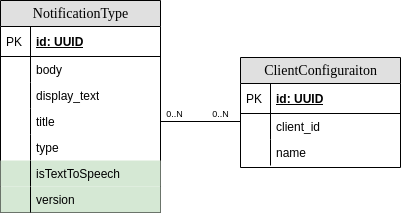
\includegraphics[width=\textwidth]{/home/joshua/FHNW/dev/IP6/IP6_Bachelorarbeit_Bericht_Cloudbasiertes_Praxisrufsystem/src/graphics/diagramms/erd_t2s_v01.drawio}}
        \caption{ERD Ausschnitt - Konfiguration Sprachsynthese}
    \end{minipage}
\end{figure}

Neben dem Feld isTextToSpeech, wird die NotificationType Entity um ein weiteres Feld ''version'' erweitert.
Das Versionsfeld beinhaltet eine Ganzzahl welche mit jeder Änderung inkrementiert wird.
Der Inhalt dieses Felds wird ebenfalls beim Versenden von Benachrichtigungen mitgesendet.
Auf Client-Seite wird diese Information zur Implementierung eines Cache verwendet.

\clearpage
\subsubsection{Integration Sprachsynthese Provider}

Dieses Kapitel beschreibt, wie Amazon Polly in das cloudbasierte Praxisrufsystem integriert wird, um das Vorlesen von Benachrichtigungen zu ermöglichen.

Die Anbindung an Amazon Polly erfolgt zentral im Cloudservice.
Sämtliche Anfragen an Amazon Polly werden durch den Cloudservice gemacht.
Empfänger von Benachrichtigungen senden keine direkten Anfragen an Amazon Polly.
Sie kommunizieren stattdessen mit dem Cloudservice.
Dieser führt die Anfrage an Amazon Polly aus und gibt die Resultate an den Anfrager zurück.

Für die Anbindung von Amazon Polly wird der Cloudservice um ein Modul mit dem Namen ''Speech Synthesis'' erweitert.
Dieses Modul muss unabhängig von allen anderen Domänen-Modulen des Cloudservice umgesetzt werden.
Werden Daten aus einer anderen Domäne benötigt, muss die Kommunikation über die REST API des entsprechenden Domänen-Moduls gehen.
Diese Unabhängigkeit ermöglicht es, das Modul in Zukunft einfach aus dem Cloudservice auszubauen und als eigenständigen Microservice zu betreiben.

Die Abhängigkeit zu Amazon Polly als Provider soll weitmöglichst minimiert werden.
So kann bei Bedarf einfacher auf einen anderen Provider gewechselt werden.
Um dies zu ermöglichen wird das Interface SpeechSynthesisService definiert.
Dieses gibt eine einzelne Methode vor, welche eine InputStreamResource zurückgibt und eine Universal Unique Id (UUID) als Parameter entgegennimmt.
Der Parameter entspricht der technischen Identifikation des zu synthetisierenden Benachrichtigungstypes (NotificationType).
Die InputStreamResource muss die synthetisierten Sprachdaten enthalten.
Dieses Interface wird der Komponente, welche die Schnittstelle nach aussen bietet verwendet.
Um einen neuen Provider zu unterstützen, kann dieses Interface implementiert werden und die neue Implementation in Schnittstelle verwendet werden.
Das Klassendiagramm in Abbildung 7.10 gibt einen Überblick über den Aufbau des Moduls Speech Synthesis.

\begin{figure}[h]
    \centering
    \begin{minipage}[b]{1\textwidth}
        \fbox{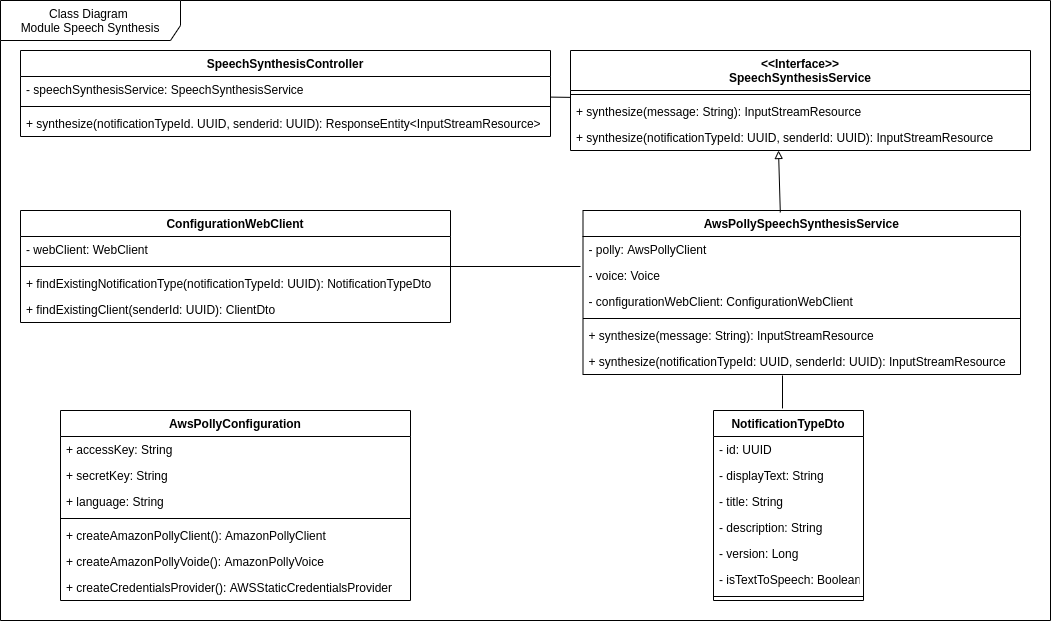
\includegraphics[width=\textwidth]{/home/joshua/FHNW/dev/IP6/IP6_Bachelorarbeit_Bericht_Cloudbasiertes_Praxisrufsystem/src/graphics/diagramms/Class_AWS_Polly_Configuration_V02}}
        \caption{Klassendiagramm Modul SpeechSynthesis}
    \end{minipage}
\end{figure}

Für die Anbindung des Providers Amazon Polly wird das SpeechSynthesisService Interface mit der Klasse AwsPollySpeechSynthesisService implementiert.
Amazon stellt einen Java Bibliothek für Amazon Polly zur Verfügung, welcher diese Anbindung ermöglicht~\cite{aws_polly_sdks}.
Diese Bibliothek bietet alle Klassen die für die Anbindung an AWS Polly nötig sind und wird in der Implementierung des SprachSyntheseProviderService verwendet, um den Service anzubinden.

Die Anbindung von Amazon Polly benötigt drei Komponenten.
Als Erstes muss eine Instanz von AWSStaticCredentialsProvider zur Verfügung gestellt werden.
Dieser liefert die Credentials, welche das System berechtigen, Anfragen an AWS Polly zu senden.
Als Zweites muss eine Voice konfiguriert werden.
Die Voice definiert Sprache und Stimme, welche für die Sprachausgabe verwendet wird.
Letztlich muss eine Instanz von AmazonPollyClient konfiguriert werden.
Dieser Client wird verwendet, um Anfragen an AWS Polly zu senden.
Er verwendet den zuvor konfigurierten CredentialsProvider, um die Anfrage mit den entsprechenden Credentials zu ergänzen.
Die zuvor konfigurierte Voice wird bei Anfragen an Amazon Polly mitgesendet, damit die Daten mit den gewünschten Parametern synthetisiert werden.

Der Cloudservice ist als Java-Applikation mit Spring Boot umgesetzt.
Dies ermöglicht es, die notwendigen Komponenten in einer Spring Konfigurationsklasse zu konfigurieren und als Spring Beans zu instanziieren.
Über die Dependency Injection von Spring werden diese Komponenten dem AwsPollySpeechSynthesisService übergeben werden.

Die Properties, welche für die technische Konfiguration notwendig sind, werden aus dem application.yml für das aktuell aktive Profil geladen.
Sprache und Region werden sich im Rahmen dieses Projektes nie ändern und beinhalten keine sensitiven Informationen.
Sie werden deshalb direkt in der Konfigurationsdatei application.yml definiert und mit dem Quellcode des Projektes verwaltet.
Als Credentials für die Anbindung dienen die zwei Schlüssel AccessKey und SecretKey.
Diese werden nicht direkt im application.yml abgelegt.
Für sämtliche Credentials wird im application.yml ein Platzhalter definiert, welcher die Credentials aus entsprechend benannten Umgebungsvariablen lädt.
Die Zugangsdaten müssen damit nicht mit dem Quellcode verwaltet werden.

\subsubsection{Schnittstelle Cloud Service}

Endgeräte im Praxisrufsystem müssen Sprachdaten über den Cloudservice beziehen können.
Das Modul Speech Synthesis stellt deshalb eine Schnittstelle zur Verfügung, über welche Sprachdaten abgefragt werden können.
Dabei ist es nicht möglich beliebige Textdaten in Sprachdaten zu verwandeln.
Stattdessen erlaubt der Endpunkt die Abfrage Sprachdaten für die aktuellste Version eines Benachrichtigungstypen (NotificationType).

Für die Sprachsynthese wird das Feld ''title'' auf aus der Entität NotificationType aus der Domäne Configuration verwendet.
Der Endpunkt zum Bezug von Sprachdaten nimmt deshalb einen Parameter mit dem Namen 'notificationTypeId' entgegen.
Dieser Parameter muss dem technischen Identifikator eines Benachrichtigungstyps (NotificationType) entsprechen.
Anhand dieses Identifikators wird der entsprechende NotificationType über die API des Moduls Configuration bezogen.
Anschliessend wird eine Anfrage an Amazon Polly gesendet um die Textdaten als Sprache zu synthetisieren.
Die von Polly gelieferten Sprachdaten können anschliessend als Resultat zurückgegeben werden.

Der Endpunkt für die Abfrage von Sprachdaten im Cloud Service wird als Spring RestController umgesetzt.
Die Sprachdaten werden dabei als Binärdaten mit Media Type ''audio/mp3'' im Body der Response zurückgegeben.
Der Endpunkt wird aus Endgeräten mit Http GET Anfragen angesprochen.

\clearpage
\subsubsection{Anbindung Mobile Client}

Dieses Kapitel beschreibt wie die API des Cloudservice aus einer nativen iOS Applikation abgesprochen werden kann.

Für die Integration des SpeechSynthesis Endpunkts aus dem CloudService wird die in Kapitel 7.2 beschriebene Klasse PraxisrufApi erweitert.
Neben dem Abfragen von JSON Daten über HTTP Schnittstellen, muss diese für die Sprachsynthese auch das Herunterladen von Dateien unterstützten.
Dazu wird die Komponente URLSession aus der iOS Standardbibliothek verwendet.
Diese bietet mit URLSession.downloadTask die Möglichkeit Inhalte von einer URL herunterzuladen~\cite{ios_downloadtask}.

Der Service PraxisrufApi wird dementsprechend um eine Methode mit dem Namen ''download'' ergänzt.
Diese ist dafür verantwortlich, eine Anfrage für den Download mit Credentials aus dem iOS Keystore zu ergänzen und die Abfrage zu versenden.
Die Resultate der Abfrage und aufgetretene Fehler werden analog zu anderen Abfragen an eine Callback-Funktion übergeben.
Heruntergeladene Dateien werden von PraxisrufApi in einem temporären Verzeichnis gespeichert.
Das Resultat im Erfolgsfall ist deshalb nicht die heruntergeladene Datei selbst, sondern eine URL welche auf die Datei im temporären Verzeichnis zeigt.

Die Sprachsynthese für Benachrichtigungen muss automatisch ausgeführt werden, nachdem eine relevante Benachrichtigung empfangen wurde.
Der Empfang der Benachrichtigung findet über die Anbindung von Firebase Cloud Messaging im AppDelegate statt.
Die Benachrichtigung wird im AppDelegate empfangen und an die Applikation übergeben.
Die empfangene Benachrichtigung beinhaltet mit dem ''isTextToSpeech'' Flag, die Information, ob sie für die Sprachsynthese relevant ist.

Ist eine Benachrichtigung für Sprachsynthese relevant, werden die Sprachdaten dazu vom Cloudservice bezogen.
Dazu wird ein SpeechSynthesisService implementiert, welcher PraxisrufApi verwendet, um eine Anfrage an den Cloudservice zu senden.
Wurden die Daten erfolgreich geladen, kopiert der SpeechSynthesisService die heruntergeladenen Daten aus dem temporären Downloadverzeichnis in ein permanentes Verzeichnis.
Die Datei wird dabei unter dem Namen ''$<$NotificationTypeId$>$''.''$<$Version$>$'' gespeichert.
Sowohl NotificationTypeId als auch Version können der empfangenen Benachrichtigung entnommen werden.
Nachdem die Sprachdatei unter dem neuen Namen gespeichert ist, wird ihr Inhalt abgespielt.

Die Namenskonvention für die gespeicherten Sprachdateien, erlaubt es ein Cache auf der Seite der iOS Applikation umzusetzen.
Bevor der SpeechSynthesisService eine Anfrage an den Cloudservice absetzt, prüft er, ob bereits eine Datei mit dem entsprechenden Namen vorhanden ist.
Ist dies der Fall, wird keine Anfrage an den Cloudservice gesendet und es wird die bereits gespeicherte Sprachdatei abgespielt.
Dieses Cache ermöglicht es Anfragen für Sprachsynthese zu minimieren und nach Änderungen trotzdem immer die aktuellsten Daten zu erhalten.

\clearpage
\subsubsection{Laufzeitsicht}

Dieses Kapitel fasst den Ablauf für das Senden, Empfangen und Vorlesen von Benachrichtigungen zusammen.

Um eine Benachrichtigung zu versenden, sendet ein Mobile Client eine Anfrage an den Cloudservice.
Dieser lädt die gespeicherte Konfiguration und findet alle für die gewünschte Benachrichtigung relevanten Empfänger.
Anschliessend erstellt er für jeden Empfänger eine Benachrichtigung und versendet diese über den Messaging Service.
Der Messaging Service stellt die Benachrichtigungen an die Empfänger zu~\cite{ip5}.

Benachrichtigungen werden im Mobile Client über die Anbindung an den Messaging Service im AppDelegate empfangen.
Im AppDelegate werden die Informationen aus der empfangenen Benachrichtigung gelesen und in das interne Model der Mobile Client Applikation überführt.
Anschliessend wird die Benachrichtigung an das Betriebssystem übergeben damit auf dem Gerät ein Benachrichtigungston abgespielt und eine Push-Benachrichtigung angezeigt wird.
Daraufhin wird die Benachrichtigung im internen Model einem NotificationService übergeben.
Dieser fügt die empfangene Benachrichtigung in eine Inbox ein.
Ab diesem Moment ist die Benachrichtigung in der Inbox des Mobile Clients ersichtlich.

\begin{figure}[h]
    \centering
    \begin{minipage}[b]{0.9\textwidth}
        \fbox{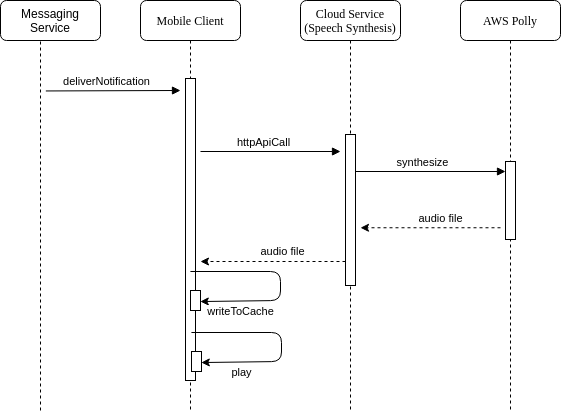
\includegraphics[width=\textwidth]{graphics/diagramms/Sequence_Speech_Synth_V01}}
        \caption{Sequenzdiagramm Sprachsynthese - Systemsicht}
    \end{minipage}
\end{figure}

Nachdem eine empfangene Benachrichtigung der Inbox hinzugefügt wurde, wird geprüft ob Sprachsynthese in den lokalen Einstellungen aktiviert ist.
Ist diese deaktiviert, endet die Verarbeitung.
Ist die Sprachsynthese lokal aktiviert, wird geprüft ob das ''isTextToSpeech'' Flag auf der Benachrichtigung aktiviert ist.
Nur wenn das Flag aktiviert ist, wird die Benachrichtigung an den SpeechSynthesisService übergeben.
Der SpeechSynthesisService prüft als erstes, ob die Sprachdaten für die empfangene Benachrichtigung bereits lokal zur Verfügung stehen.
Dies wird gemacht in dem er überprüft, ob im Applikationsverzeichnis bereits eine Datei für Id und Version der Benachrichtigung vorhanden ist.
Ist dies der Fall, werden die Inhalte dieser Datei abgespielt und es wird keine Anfrage an den Cloudservice versendet.
Wenn die Daten gar nicht oder nur in einer anderen Version lokal gefunden werden, wird eine Anfrage an den CloudService gesendet.

Sobald Sprachdaten über die Cloudservice API angefragt werden, lädt dieser die Inhalte der relevanten Benachrichtigung aus der Konfiguration.
Anschliessend sendet der Cloudservice eine Anfrage an Amazon Polly, um den Titel der Benachrichtigung als Sprachdaten zu synthetisieren.
Die Resultate von Amazon Polly werden als Resultat der Anfrage des Mobile Clients zurückgegeben.
Der Client speichert die empfangenen Daten lokal im Applikationsverzeichnis unter Id und Version verknüpften NotificationType.
Nachdem die Daten gespeichert wurden, wird deren Inhalt abgespielt.

\clearpage
